\chapter{Results and Discussion}
\label{chap:Results}
Since a large part of our bachelor task consisted of face image quality research, this chapter is of great importance. After conducting the experiments in Chapter \ref{chap:subjective}, we gathered large amount of data, which we had to process. This data will be presented in the form of statistical calculations, such as box plots, correlation graphs and standard deviation graphs. The main goal of the chapter is to tie together the results we achieved in the objective and subjective face quality assessment, discuss them and present an in-depth look into the performance of the FIQMs relative to our collected ground truth data.   

\section{Main Experiment}
The results we achieved are split into two sections. In this first section the results of the objective assessment and our first subjective experiment will be presented and discussed. Both assessment categories are based on the three datasets provided by Mobai, which were described in Chapter \ref{chap:subjective}. 
%Utfylle mer her senere om hvordan seksjonen er oppbygd.

\subsection{Objective Assessment Scores}
The FIQMs presented in Chapter \ref{chap:FQA} use different approaches to predict the perceived face quality. Their predicted perception of quality is supposed to correlate with human assessment, which is the whole purpose of the metrics. The objective predictions produced by the FIQMs were measured up to human assessment to evaluate how true to their purpose they were. This evaluation was carried out by comparing the results of the FIQMs against the results gathered from human observers. The same resized images used in our first subjective experiment were used as input to our two FIQMs. 
\newpage

\begin{figure}[h]
\centering
    \subfloat[Combined passport alike]
        {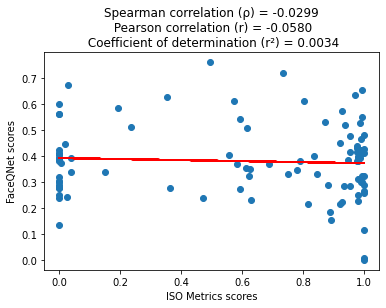
\includegraphics[scale = 0.36]{figures/ISO_FaceQNet1.png}\label{fig:combinedpassportalikeplot}}
    \subfloat[Capture from photo]
        {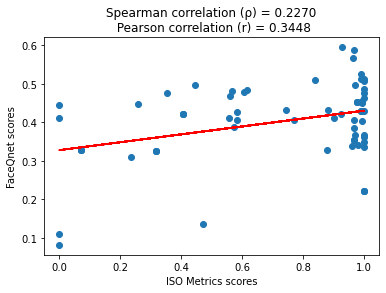
\includegraphics[scale = 0.36]{figures/ISO_FaceQNet2.png}\label{fig:capturefromphotoplot}}
    \subfloat[Selfie dataset]
        {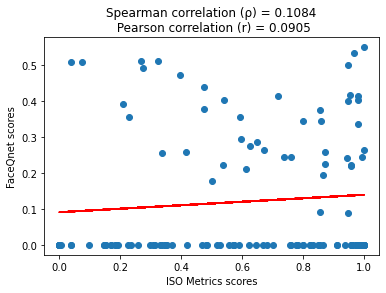
\includegraphics[scale = 0.36]{figures/ISO_FaceQNet3.png}\label{fig:selfiedatasetplot}}
    \caption{2D correlation graphs of the scores provided by the FIQMs on the three datasets with ISO Metrics scores along the x-axis and FaceQNet scores along the y-axis. The Spearman and Pearson correlation, including the coefficient of determination, are calculated as well.}
    \label{fig:corrFIQMs}
\end{figure}

The three plots depicted in Figure \ref{fig:corrFIQMs} show the scores of each image, which are represented by dots, in the three datasets. One can easily see the large difference in scores predicted by the two FIQMs. In regards to the first plot, with the ``Combined passport alike'' dataset, ISO Metrics had a large gap between the ratings provided. Most of the images were given a score above 0.9, while some received the lowest score of zero. Images with a score of zero provided by ISO Metrics were usually of faces where both eyes were not visible. ISO Metrics is coded in such a way that facial images where both eyes are not visible will be filtered out and provided with a score of zero. FaceQNet however, rated the images far more evenly between the 0.2 and 0.6 range. Figure \ref{fig:capturefromphotoplot} shows far more evenly distributed scores even though the scores from FaceQNet were significantly lower than ISO Metrics. As for Figure \ref{fig:selfiedatasetplot} the scores from ISO Metrics were equally spread from zero to one, where as most of the FaceQNet scores were zero. The images rated zero were mostly because the cropping part of FaceQNet failed. The images were therefore manually provided a score of zero. In other words, FaceQNet is not a suitable FIQM for the Selfie-dataset.  

The sample Pearson correlation coefficient ($r$) was calculated as: 
\begin{equation}
    {\displaystyle r={\frac {\sum _{i=1}^{n}(x_{i}-{\bar {x}})(y_{i}-{\bar {y}})}{{\sqrt {\sum _{i=1}^{n}(x_{i}-{\bar {x}})^{2}}}{\sqrt {\sum _{i=1}^{n}(y_{i}-{\bar {y}})^{2}}}}}}
\end{equation}
where $n$ is the sample size, $x_{i}$ and $y_{i}$ denotes the individual sample points (scores) from ISO Metrics and FaceQNet respectively while ${\bar {x}}={\frac {1}{n}}\sum _{i=1}^{n}x_{i}$ and ${\bar {y}}={\frac {1}{n}}\sum _{i=1}^{n}y_{i}$ represents the sample means from both FIQMs. Another type of correlation coefficient, the Spearman rank correlation coefficient ($\rho$) \cite{wiki:spearman} was also calculated because it does not assume that both variables are normally distributed.

As for the plots depicted in Figure \ref{fig:corrFIQMs} one can see that a correlation between ISO Metrics and FaceQNet on the three datasets was near no existent. Figure \ref{fig:capturefromphotoplot} showed the closest to zero correlation between the datasets. The $\rho$ and $r$-values even show a negligible negative correlation which is confirmed by the red linear regression line which slightly points downwards. On the contrary Figure \ref{fig:capturefromphotoplot} showcases a $r$-value of 0.34 which is still considered a weak correlation, but is noticeably higher than the two other datasets. !!!The reasoning for this is because of the??? . The rightmost plot is similar to plot (a), but with a negligible positive correlation. It is highly likely that if FaceQNet had worked for the dataset, the correlation would be different. 


\subsection{Subjective Assessment Scores}
As earlier mentioned, the first subjective experiment was supposed to gather ground truth data about each of the three datasets provided by Mobai. These datasets were equally split and mixed amongst the three survey sessions. Since the survey sessions consisted of images from all datasets, the data gathered from each survey session had to be organized and matched with the images of the corresponding dataset. That way the ground truth data could be analyzed on the original datasets and not on the datasets used for each survey session.

\begin{figure}[h]
    \centering
    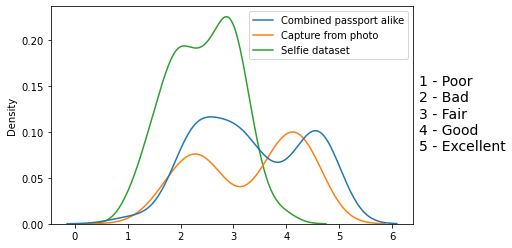
\includegraphics[width=0.7\textwidth]{figures/KernelPlots.png}
    \caption{Kernel density estimation on the subjective scores on each dataset. There is a clear difference between the quality of the Selfie dataset vs the two others.}
    \label{fig:kerneldensity}
\end{figure}

As shown in Figure \ref{fig:kerneldensity} one can see how the subjective opinions were distributed between the datasets. The quality of the images in the Selfie dataset were more consistent than the two other datasets, because it is more evenly distributed.   


\subsubsection*{Combined Passport Alike}


\begin{figure}[h]
    \centering
    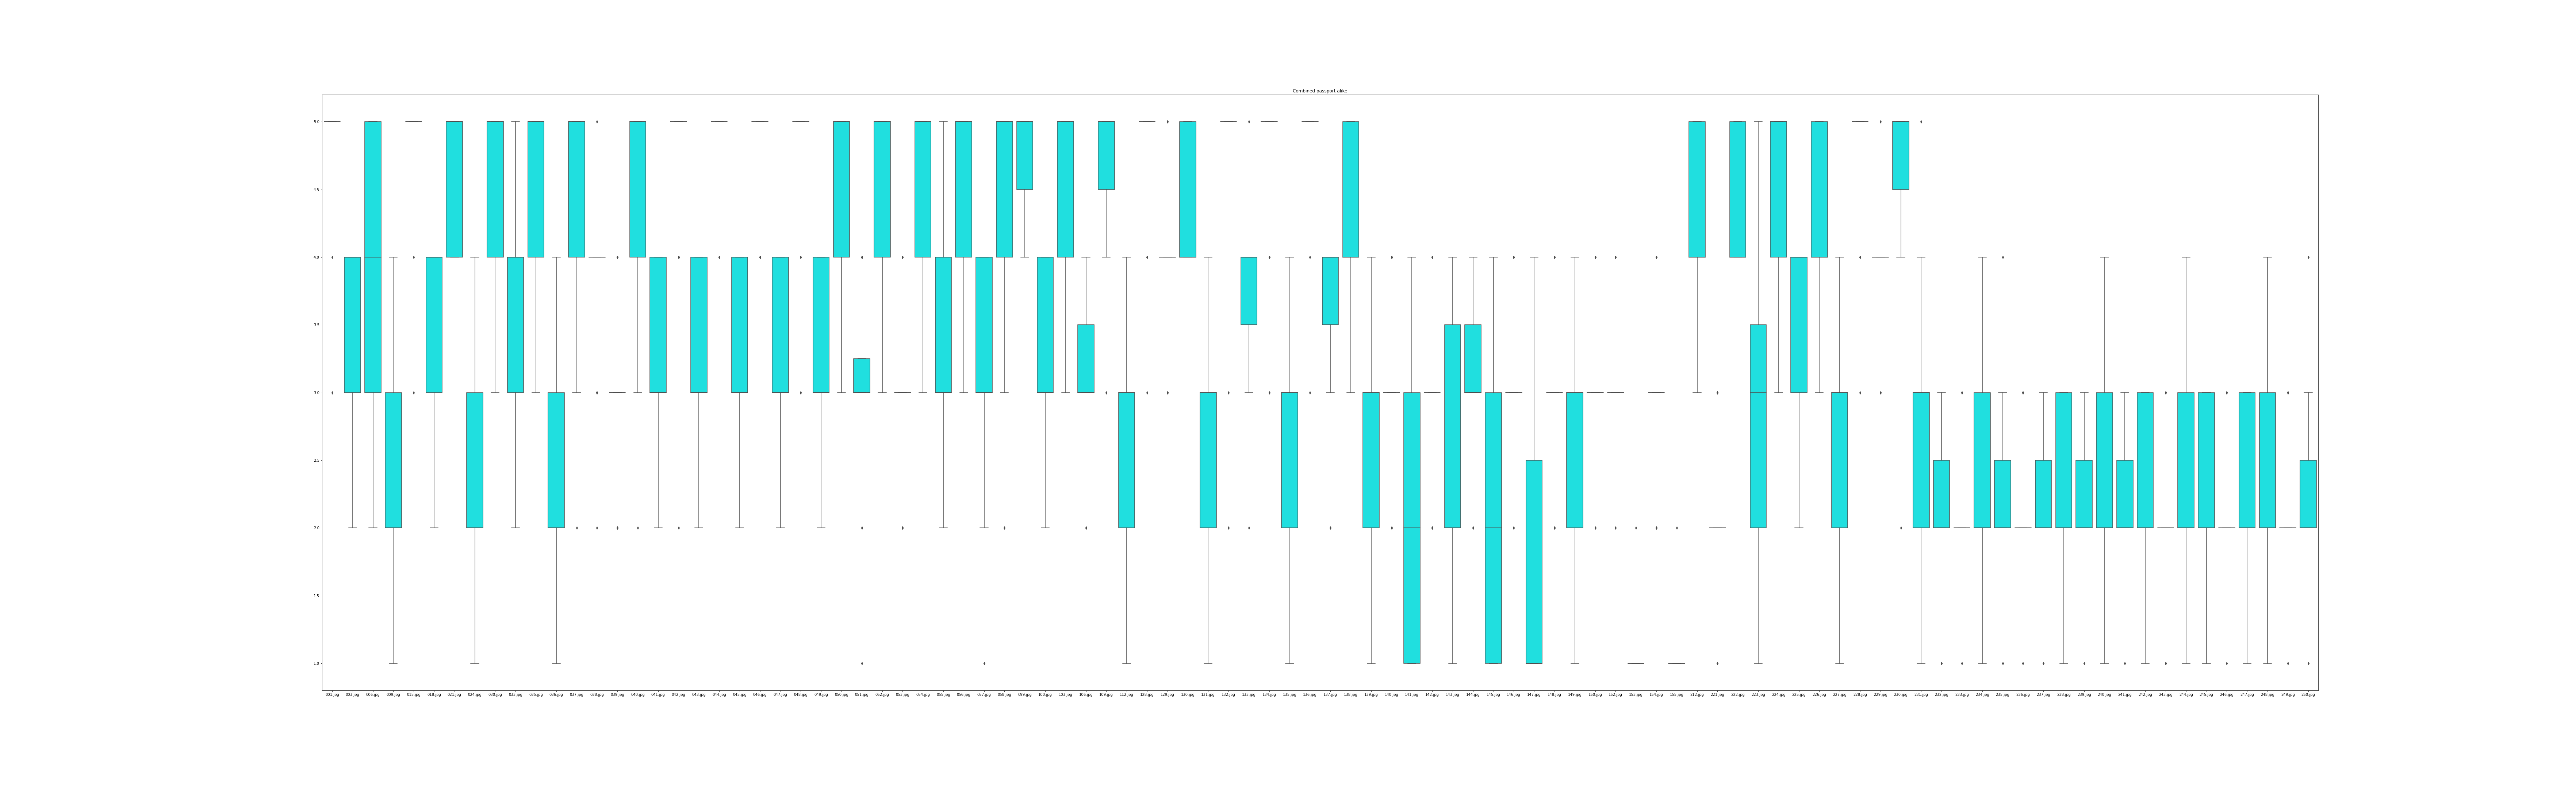
\includegraphics[width=1.0\textwidth]{figures/boxplot1.png}
    \caption{A standard box plot of the images in the ``Combined passport alike'' dataset. It shows outliers, the min and max whiskers, the first and third quartile as well as the median of the ground truth data produced by the survey participants.}
    \label{fig:boxplot1}
\end{figure}

\subsubsection*{Capture from Photo}
\begin{figure}[h]
    \centering
    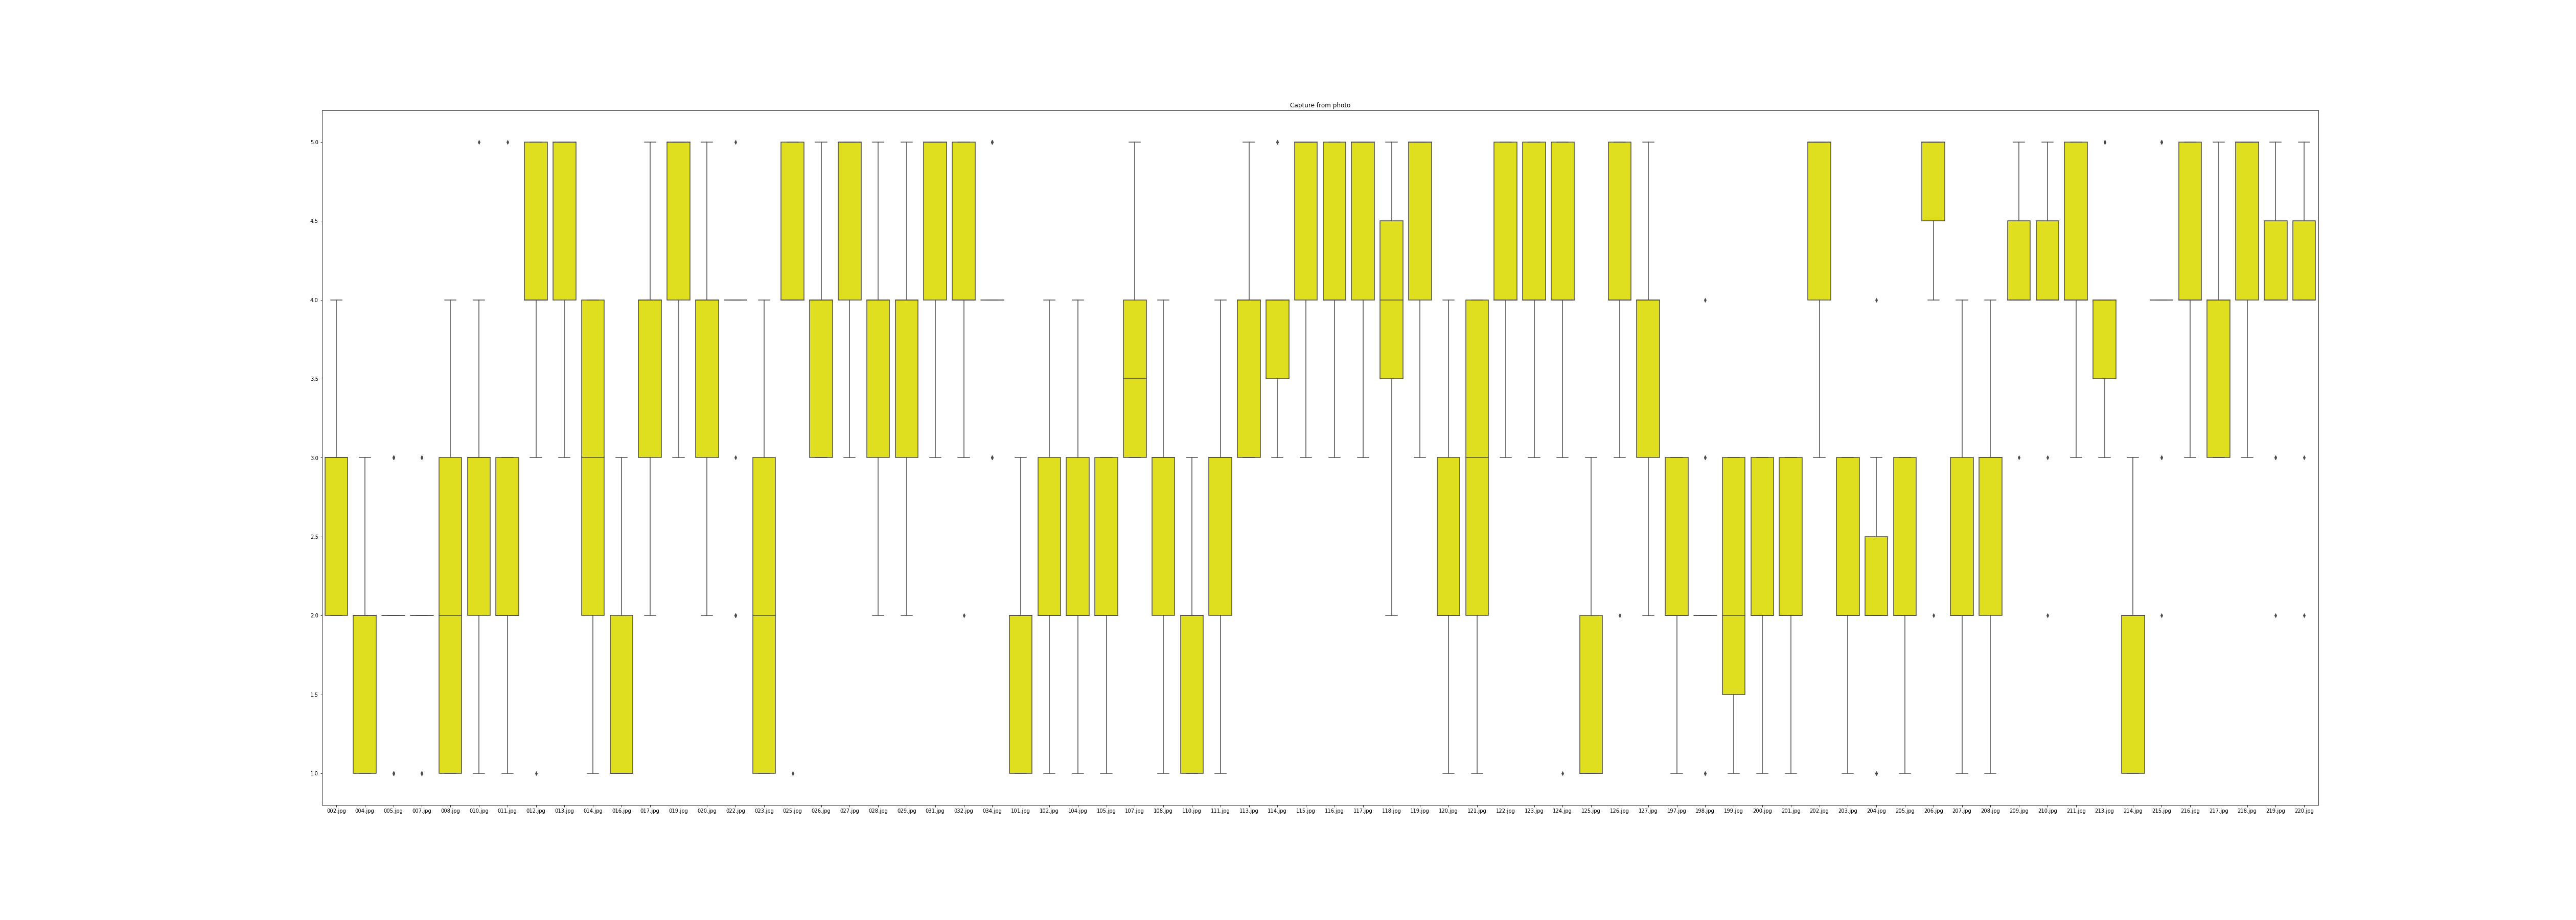
\includegraphics[width=1.0\textwidth]{figures/boxplot2.png}
    \caption{A standard box plot of the images in the ``Combined passport alike'' dataset. It shows outliers, the min and max whiskers, the first and third quartile as well as the median of the ground truth data produced by the survey participants.}
    \label{fig:boxplot2}
\end{figure}

\subsubsection*{Selfie Dataset}
\begin{figure}[h]
    \centering
    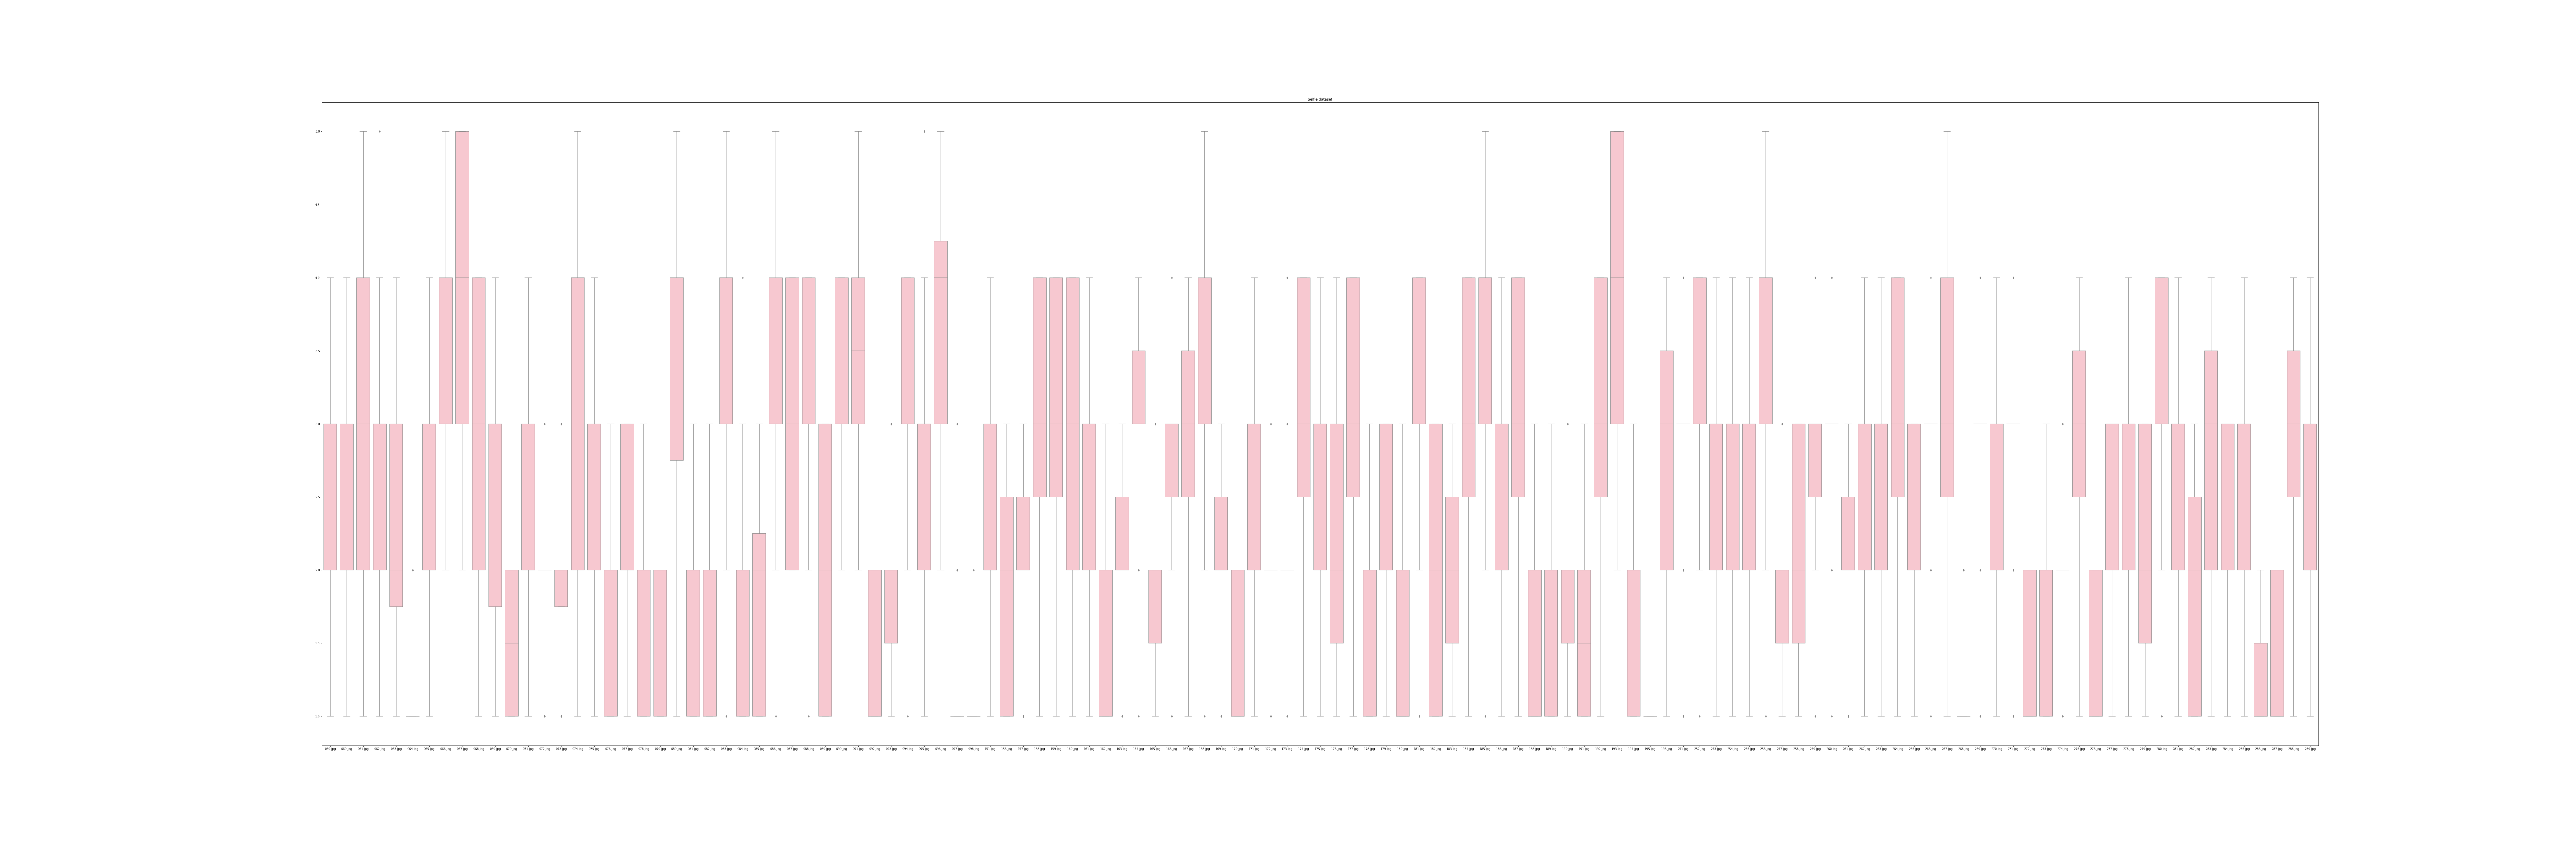
\includegraphics[width=1.0\textwidth]{figures/boxplot3.png}
    \caption{A standard box plot of the images in the ``Combined passport alike'' dataset. It shows outliers, the min and max whiskers, the first and third quartile as well as the median of the ground truth data produced by the survey participants.}
    \label{fig:boxplot3}
\end{figure}

\subsection{FIQMs vs Ground Truth Data}

\section{Second Experiment}
This second section is about the second subjective experiment we conducted based on our own dataset of 250 images. 
\subsection{Objective Assessment Scores}
\subsection{Subjective Assessment Scores}